\documentclass{article}
\usepackage{graphicx}
\usepackage{amsmath}
\usepackage{hyperref}
\usepackage{cleveref}

\graphicspath{{figs/}}

\begin{document}
\title{Analysis of FFL models}

\section{Saturating Activator}

We initially modify LEGI by adding a saturating term to the production of
activator, \cref{eqn:Asig}.
This produces a steady state activation profile that is bounded, \cref{fig:ssAI}.
The resulting response (\cref{fig:ssR}) becomes dependent on input strength
and activator nonlinearity. 

\begin{align}
    a'[t] &= \frac{ S^n }{ Km^n + S^n } - a(t) \label{eqn:Asig}\\
    i'(t) &= \alpha * ( S - i(t)) \\
    r'(t) &= \beta * ( a(t) ( R_{tot} - r(t) ) - i(t) r(t) )
\end{align}

\begin{itemize}
    \item for $Km \ll S$, it's the original LEGI model. $a$ and $i$  are equal
        for all inputs, therefore the response is flat.
    \item for $Km \approx S$ and $n=1$, saturated activator. The inhibitor
        gradually out-produces the activator, leading to a monotonically
        decreasing response. 
    \item for $Km \approx S$ and $n>1$, sigmoidal activator. The activator
        initially lags the inhibitor before attempting to catch up, producing a
        biphasic response.
\end{itemize}

\begin{figure}
    \centering
    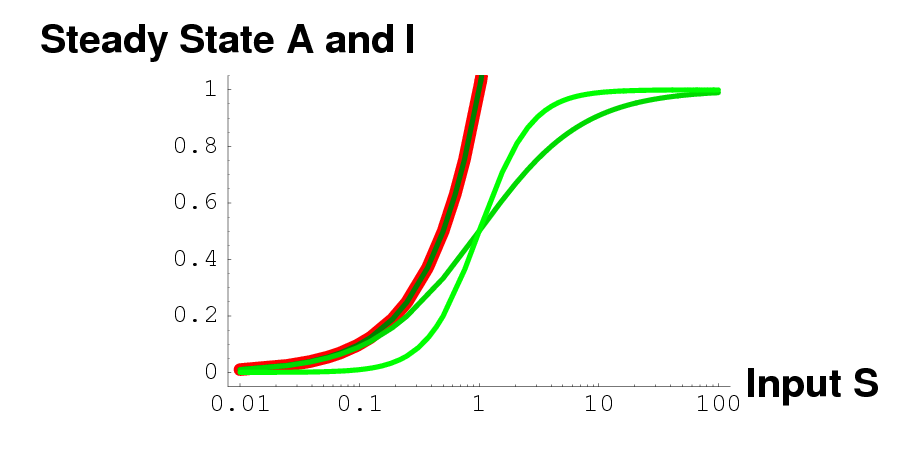
\includegraphics[width=0.9\textwidth]{ssAIR.png}
    \caption{Steady state activator, nonconserved (dark green),
        saturating (green), sigmoidal (lime) and steady state,
        nonconserved inhibitor (red). \label{fig:ssAI}}
\end{figure}


\begin{figure}
    \centering
    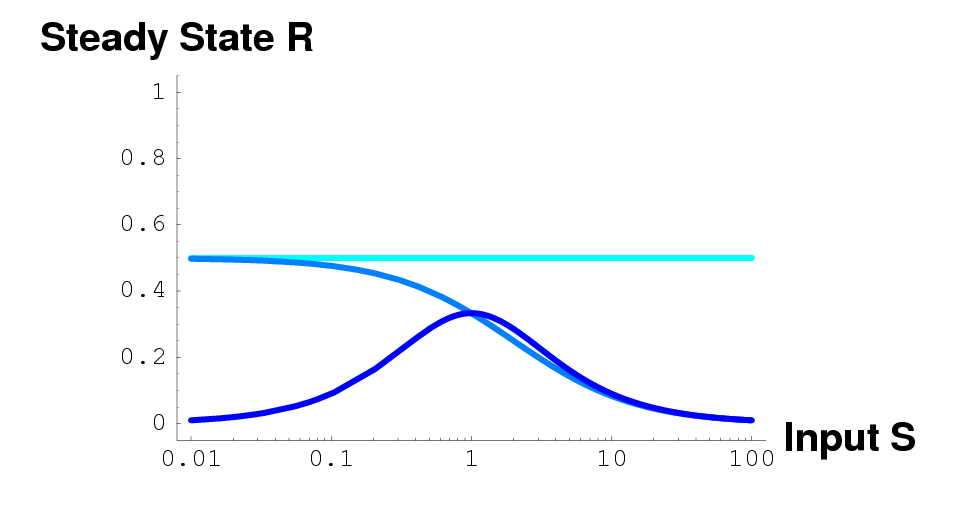
\includegraphics[width=0.9\textwidth]{ssR.png}
    \caption{Steady state response for LEGI (cyan),
        saturating activator (blue), sigmoidal activator (navy).
        \label{fig:ssR}}
\end{figure}

Looking at the response curves \cref{fig:ssR}, 
one can infer the gradient response 
in a purely local model (no diffusion of inhibitor). 
\begin{itemize}
    \item the LEGI model (cyan flat) cannot sense gradients
    \item the saturated activator (blue decreasing) can only model repulsion
    \item the sigmoidal activator (navy bell) is capable of attraction and
        repulsion 
\end{itemize}

Many metrics were then derived in an attempt to quantify ``attraction'' and
``repulsion''.
The $M_2$ metric (\cref{eqn:m2}) offered the best anti-symmetrical curve 
(\cref{fig:metric}) given the symmetrical response (\cref{fig:ssR}: navy, bell
curve). It reveals a ``stopping point'' where attraction becomes repulsion,
regardless of external gradient.

\begin{align}
    M_2 &= \frac{ r_{front} - r_{back} }{ Mean[r] } \label{eqn:m2}
\end{align}

\begin{figure}
    \centering
    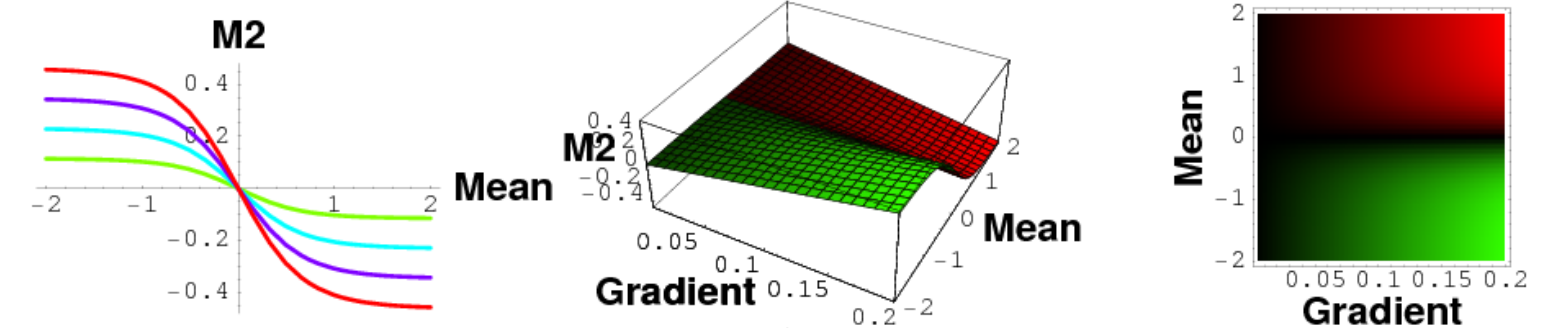
\includegraphics[width=0.9\textwidth]{metric.png}
    \caption{Chemotaxis metric \label{fig:metric}}
\end{figure}

\section{Saturating Activator, diffusible inhibitor}

Here we modify LEGI by adding a saturating term to the production of
activator, \cref{eqn:Asat} and allowing for the diffusion of inhibitor,
\cref{eqn:Idiff}.
\begin{align}
    \frac{ \partial a(t,x) }{ \partial t } &= S * (A_{tot} - a) - a
        \label{eqn:Asat} \\
    \frac{ \partial i(t,x) }{ \partial t } &= \alpha * ( S - i) +
        D_i \frac{ \partial^2 i}{ \partial x^2 } \label{eqn:Idiff} \\
    \frac{ \partial r(t,x) }{ \partial t } &= \beta * ( a ( R_{tot} - r ) - i * r )
\end{align}
Modifying the diffusion of the inhibitor $D_i$ 
transitions the model between a purely local one to a purely global model.
Applying the metric from \cref{eqn:m2} yields the response in 
\cref{fig:metricVsDi} as a function in input and inhibitor diffusion.

\begin{itemize}
    \item when $D_i \approx 0$, we have a monotonically decreasing response,
        similar to the blue curve in \cref{fig:ssR} and thus only repulsion for
        all inputs (all red in \cref{fig:metricVsDi}, for $D_i = 10^{-5}$)
    \item when $D_i \approx 1$, we interestingly achieve the same
        biphasic behavior of the purely local model with sigmoidal activation. 
    \item when $D_i \gg 1$, we almost get the original LEGI, modeling only
        attraction until the activator saturates. 
\end{itemize}

\begin{figure}
    \centering
    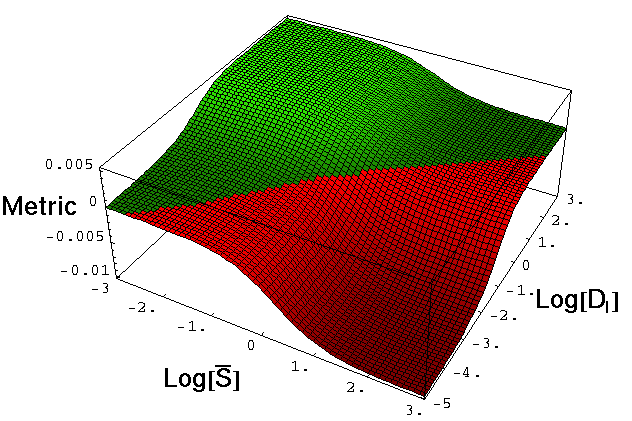
\includegraphics[width=0.9\textwidth]{MetricVsAvgVsDi.png}
    \caption{$M_2$ chemoattraction (green) and chemorepulsion (red) \label{fig:metricVsDi}}
\end{figure}




\section{Mechanical model}

The mechanical model of the cell is modeled as a series of Kelvin-Voigt
elements.  \cref{fig:tension_fig}
A Kelvin-Voigt element is a spring and damper connected in parallel that models
a visco-elastic material. Adhesion is modeled as a set of K-V elements anchored
in parallel to the ground while the cytoskeleton is modeled as a set of K-V
elements connected in series across adhesion sites. Upon applying a protrusive
force on the edge elements the internal stresses can be computed
\cref{fig:mech-t}. This internal stress can be used as feedback to the chemical
signalling.


\begin{align}
    s_i     &= L * \frac{ i-1 }{ n-1 }  \\
    x_i(0)  &= s_i \\
    x'_i(0) &= 0 \\
    m_i * x''_i(t) &= k_a (s_i - x_i(t)) - \eta_a * x_i'(t)  \\
                   &\phantom{{}=}+ Fm_i(t) + Fm_{i-1}(t) \notag \\
    Fm_i(t) &= k_m \left( \frac{ x_{i+1}(t) - x_i(t) }{ dL } - 1 \right)  \\
            &\phantom{{}=} - \eta_m \left(x_i(t) - x_{i+1}(t) \right) \notag
\end{align}

\begin{figure}
    \centering
    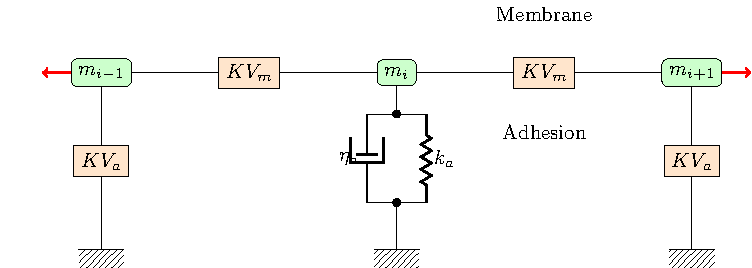
\includegraphics[width=0.9\textwidth]{./tension_fig.pdf}
    \caption{Membrane model \label{fig:tension_fig}}
\end{figure}

\begin{figure}
    \centering
    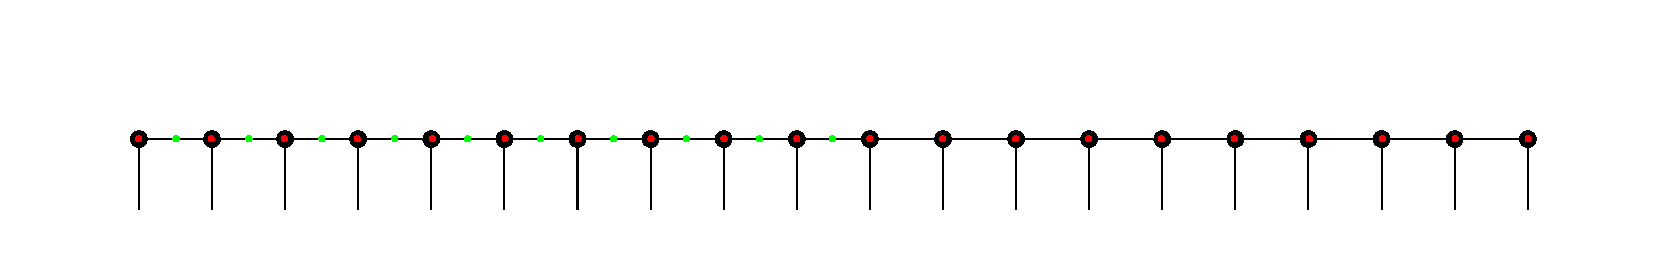
\includegraphics[width=0.9\textwidth]{mech-0.pdf}
    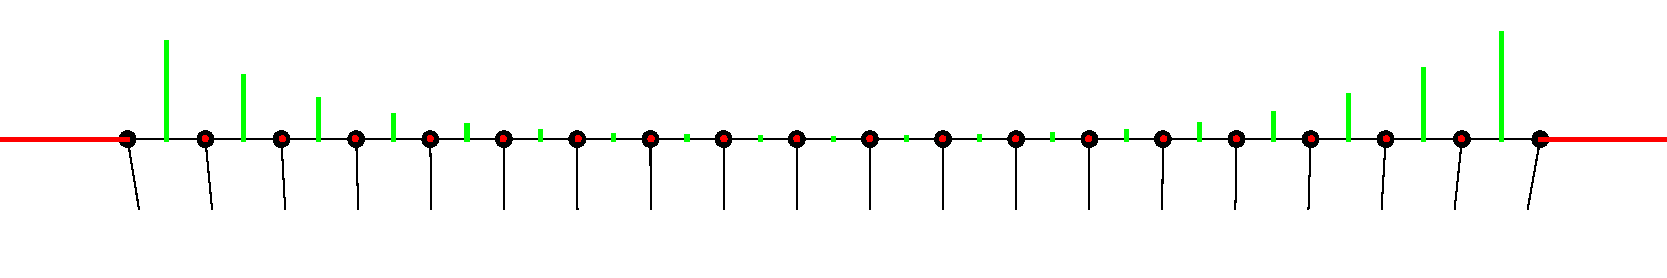
\includegraphics[width=0.9\textwidth]{mech-10.pdf}
    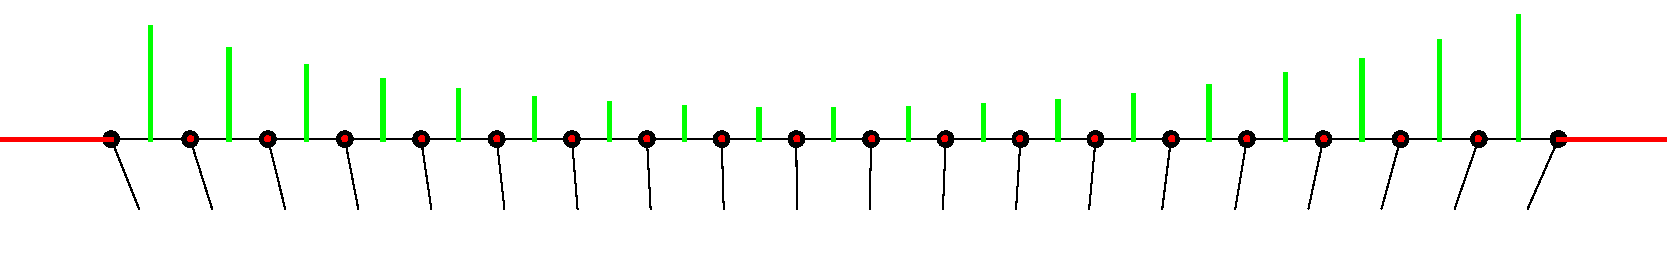
\includegraphics[width=0.9\textwidth]{mech-200.pdf}
    \caption{ Mechanical model of membrane undergoing stretching. Black lines,
        Kelvin-Voigt elements, vertical ones are adhesive elements, horizontal
        ones are cytoskeletal. Red lines, force of protrusion. Green lines, force of
        stress on spring in K-V element
        (modeling cytoskeletal elastic stretch along cell).
        \label{fig:mech-t}}
\end{figure}


\section{Notes}

\iffalse

Steady-state

\begin{align}
   a_{ss} &= A_{tot} * \frac{ S }{ 1 + S } \\
   i_{ss} &= S \\
   r_{ss} &= A_{tot} * \frac{ R_{tot} }{ 1 + S + A_{tot} } 
\end{align}

\begin{itemize}
    \item noisy gradients? 
    \item inputs varying in time
    \item inputs varying in space
\end{itemize}

neuronal migration based on a local model
\fi

\end{document}

